\section{The Landscape of Rationality for Finite Word Relations}
\label{sec:preliminaries-automatic-structures-relations}

The class of "regular languages" is remarkably stable, and can either be characterized as the 
languages recognized by either:
\begin{itemize}
	\item deterministic or non-deterministic finite state automata,
	see "eg" \cite[Proposition~1.2.3, p.~7]{Pin2021FiniteAutomata},
	\item two-way finite state automata by Shepherdson-Rabin-Scott theorem
		\cite[Theorem~2, p.~198]{Shepherdson1959ReductionTwoWay}
		\cite[Theorem~15, p.~123]{RabinScott1959FiniteAutomata},
	\item rational expressions by Kleene's theorem,
		see "eg" \cite[Theorem~1.5.11, p.~34]{Pin2021FiniteAutomata},
	\item monadic second-order logic by Trakhtenbrot-Büchi-Elgot theorem,
		see "eg" \cite[Theorem~2.2, p.~32]{Bojanczyk2020MSO}, or
	\item finite monoids,
		see "eg" \cite[\S~1.4.2, p.~19]{Pin2021FiniteAutomata}.
\end{itemize}
Moreover, all transformations between these representations are effective---although some
models can be strictly more succinct.

These equivalences explain why the terms \emph{recognizable language}---meaning implicitly
``recognizable by a finite-state automaton'' or ``recognizable by a finite monoid''---and
\emph{rational language}---meaning ``described by a rational expression''---are used 
interchangeably. In fact, in this thesis as well as in most of the literature,
we will use the generic term "regular language".
However, in more complex settings, for instance subsets of non-free monoids,%
\footnote{Recall that a language is nothing else but a subset of a free
(usually finitely-generated) monoid.}
the equivalence between these classes no longer holds. \cite{Pin2021StackExchange}

The landscape of rationality for $k$-ary relations of finite words ($k \geq 2$) is far more complex than for languages,\footnote{Which can be seen as unary relations of finite words.} as depicted in \Cref{fig:landscape-rationality-relations}. We will briefly present these classes,
although this thesis will only deal with the two most restrictive ones, namely
"recognizable@@rel" and "automatic relations".%
\footnote{It should be noted that the names
of these classes were often coined independently of one another---sometimes defying common sense.
For instance, "automatic relations" are named this way because they correspond to
the relations recognized by some model of automata...
not unlike most of the classes in \Cref{fig:landscape-rationality-relations}.
They are also sometimes named ``regular relations'', which have essentially nothing to do
with "regular functions".}

\begin{figure}
	\centering
	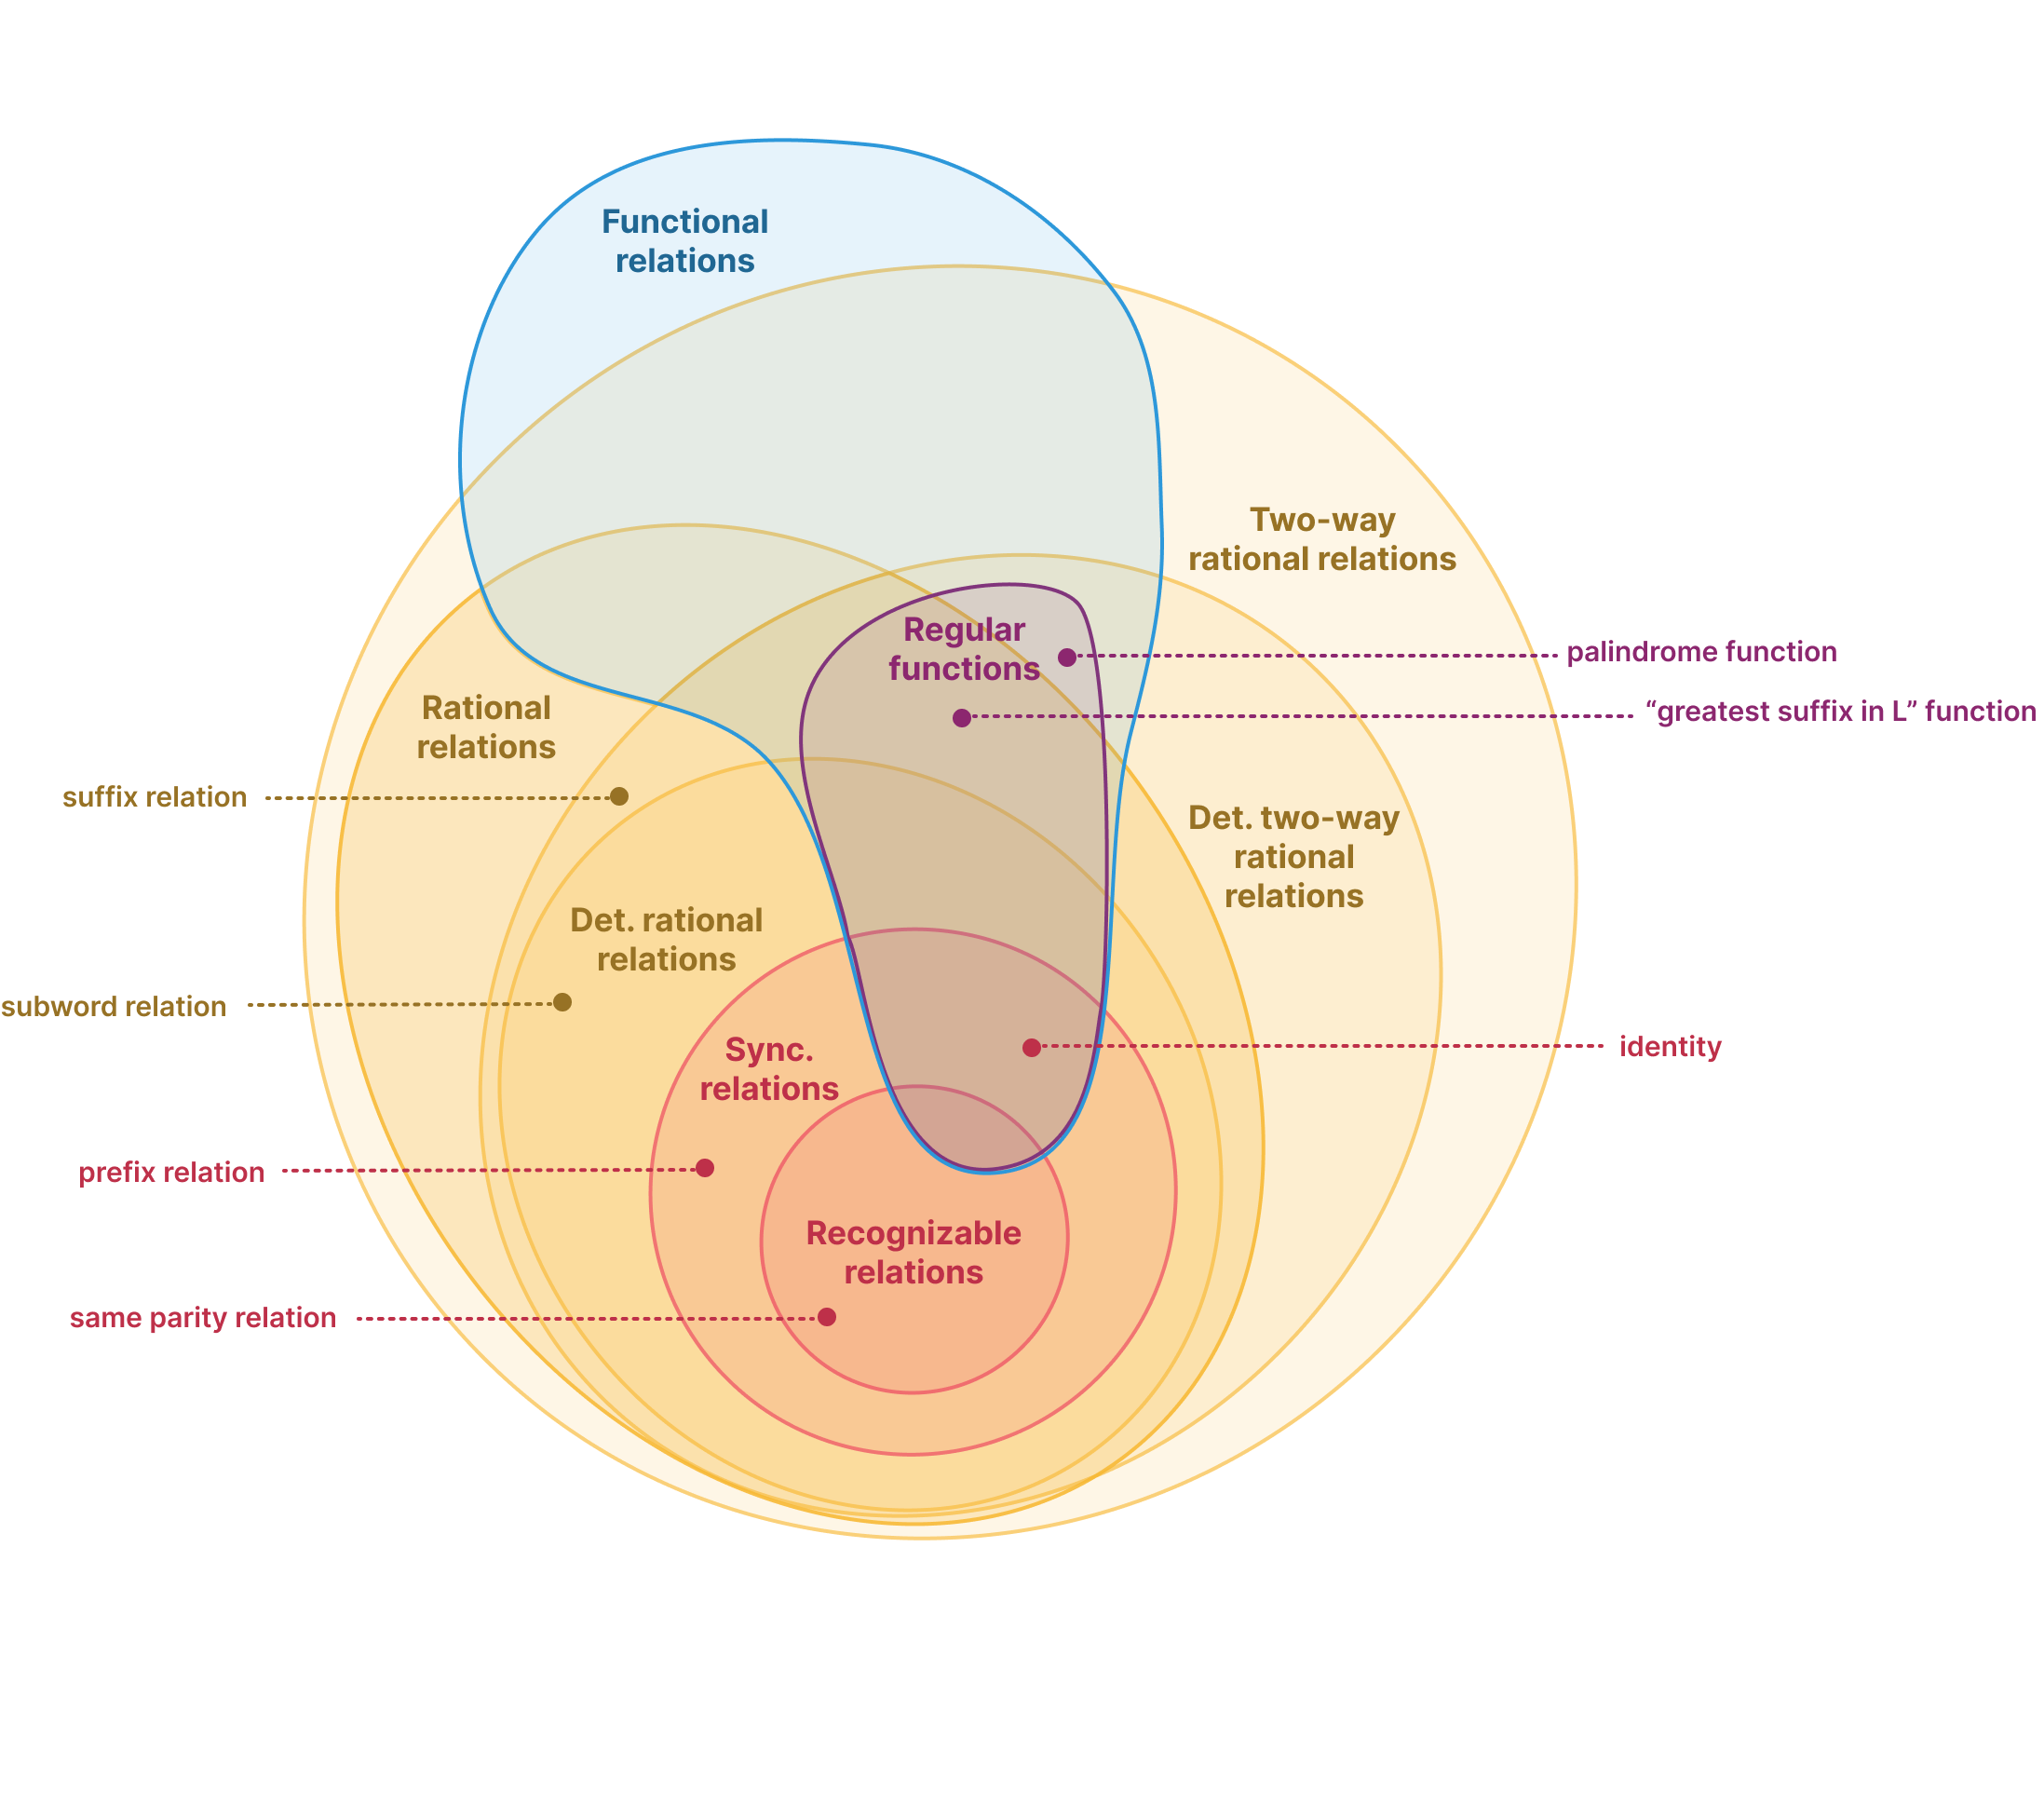
\includegraphics[width=\linewidth]{fig/landscape-rationality-relations.png}
	\caption{
		\AP\label{fig:landscape-rationality-relations}
		The ``landscape of rationality'' for binary relations.
		Dashed regions are empty.
	}
\end{figure}


\begin{itemize}
	\item todo:add polyregular functions.
	\item todo: rename ``synchronous relations'' to ``automatic relations''
	\item todo:the intersection of
	functional relations and two-way rational relations
	collapses to regular functions by
	\cite[Theorem 22, p.~243]{EH2001transduction}.
	\item cite Gaëtan's thesis (chapter 1 for finite words, chapter 8 for infinite words)
	\item mention pebble, marble and whatnot.
\end{itemize}


\begin{itemize}
	\itemAP padding symbol $\intro*\pad$
	\itemAP convolution of words $\intro*\convol$
	\itemAP convolution of a relation $\intro*\convolRel{\+R}$
	\itemAP ""automatic relation"" and $\intro*\AUT$
\end{itemize}